\documentclass[a4paper,12pt]{scrartcl} % Das Prozentzeichen fügt einen Kommentar ein.

\usepackage[ngerman]{babel} %definiert Sprache
\usepackage[left=4cm, right=2cm, top=2cm, bottom=2cm]{geometry} % definiert Ränder der Seiten
\usepackage[utf8]{inputenc}   % erlaubt Sonderzeichen
\usepackage[T1]{fontenc}        % setzt Schriftart zu T1 und erlaubt Umlaute
\usepackage{lmodern}            % verbessert Schriftart
\usepackage{microtype}          % verbessert Leerzeichen bei Nutzung von lmodern
\usepackage{amsmath,amsfonts,amssymb,amsthm}   % erlaubt Math-Umgebungen
\usepackage{graphicx}           % erlaubt das Einbinden von Grafiken
\usepackage{booktabs}           % erlaubt die Erstellung von professionellen Tabellen
\usepackage{csquotes}           % verbesserte Nutzung von Anführungszeichen
%\usepackage{longtable}          % erlaubt Tabellen, die über mehrere Seiten gehen
%\usepackage{sidewaystable}          % erlaubt die Erstellung von Tabellen im Querformat
\usepackage[labelfont=bf,format=hang]{caption} % verbesserte Beschriftung von Abbildungen und Tabellen; Das Titellabel Abbildung ist fettgedruckt. Die Sprache wird vom Babel-Paket genommen, z.B. Abbildung wenn german statt english.
\usepackage{setspace}           % erlaubt Befehle \onehalfspacing oder \doublespacing um Zeilenabstand zu definieren
\usepackage{epstopdf}           % erlaubt die Nutzung von eps-Dateien mit pdflatex
\usepackage{textcomp}           % erlaubt weitere Symbole
%\usepackage{indentfirst}       % Rückt die erste Zeile ein
\usepackage[hyphens]{url}       % setzt Zeilenumbrüche bei langen URLs (muss vor biblatex eingebunden werden)
\usepackage{enumitem}           % erlaubt benutzerdefinierte Aufzählungen

%%%% Das folgende package definiert die Nutzung von BibLaTeX für Zitationen und Literaturverzeichnisse
\usepackage[%
citestyle=authoryear-comp,%nutzt komprimierte Autor-Jahr Zitation
bibstyle=JME,% nutzt JME-style;
maxbibnames=7,% % maximale Anzahl an dargestellten Namen bevor die Akürzung mit "et al." genutzt wird
minbibnames=1, % Anzahl an genannten Autoren wenn et al. genutzt wird
maxnames=2,% maximale Anzahl an dargestellten Namen bei Zitationen before et al. genutzt wird
minnames=1,% Anzahl an genannten Autoren wenn et al. genutzt wird
datezeros=false,% keine vorstehende 0 wenn Daten dargestellt werden
date=long,%
citetracker=true, %Check ob Zitation schon einmal vorkam
isbn=false,% zeige keine ISBN im Literaturverzeichnis
url=false,% zeige keine URLs im Literaturverzeichnis
doi=true, % zeige keine DOIs im Literaturverzeichnis
eprint=false, % zeige keine eprint-Felder im Literaturverzeichnis
backend=biber % backend=bibtex ist schwächer, aber leichter zu installieren
]{biblatex}

\addbibresource{mybibfile.bib} % definiert den Namen des .bib-file	

%% Verwendung von et. al. statt u.a. im Deutschen
\DefineBibliographyStrings{ngerman}{
   andothers = {{et\,al\adddot}},
}

%% Benutzung von et al. bei mehr als 3 Autoren ab der zweiten Zitation

%http://tex.stackexchange.com/questions/48846/biblatex-et-al-beginning-from-second-citation
\usepackage{xpatch}
\AtEveryCitekey{\ifciteseen{}{\clearfield{namehash}}}

\xpatchbibmacro{cite}
  {\printnames{labelname}}
  {\ifciteseen
     {\printnames{labelname}}
     {\printnames[][1-99]{labelname}}}
  {}
  {}

\xpatchbibmacro{textcite}
  {\printnames{labelname}}
  {\ifciteseen
     {\printnames{labelname}}
     {\printnames[][1-99]{labelname}}}
  {}
  {}

\usepackage[pdfpagelabels=true,plainpages=false,pdftex,bookmarksnumbered=false,bookmarksopen=true]{hyperref}%plainpage und pdfpagelabels erlauben korrekte Abbildung links wenn verschiedene Seitennummerierungen benutzt werden
% bookmarksnumbered=false unterbindet Nummerierung im Inhaltsverzeichnis
% bookmarksopen=true öffnet das Inhaltsverzeichnis links im Adobe Reader

\hypersetup{
pdfproducer = {LaTeX},
colorlinks,
linkcolor=black,
filecolor=yellow,
urlcolor=blue,
citecolor=black,
pdftitle ={Title of the thesis},
pdfsubject ={Thesis},
pdfauthor = {Your Name },
pdfkeywords = {Some keywords}
pdfcreator={pdfLaTex}}


\usepackage[style=long,nonumberlist,acronym,automake,nomain]{glossaries} % Glossary Package für Abkürzungs und Symbolverzeichnis. Nun ist ein Glossary für Abkürzungen definiert.

\newglossary[slg]{symbolslist}{syi}{syg}{List of Symbols} %Definiert ein weiteres Glossary für Symbole.

\makeglossaries %muss nach allen Newglossary befehlen definiert werden.

%%Hier folgen die Definition von den Glossary-Einträgen der Abkürzungen

\newacronym{acro:GDP}{GDP}{Gross Domestic Product} % definiert das Akronym GDP

\newacronym{acro:OLS}{OLS}{Ordinary Least Squares} % definiert das Akronym OLS
\glsadd{acro:OLS} % Liste das Akronym im Abkürzungsverzeichnis auch wenn es im Dokument nicht genutzt wurde

%%Hier folgen die Definitionen von den Glossary-Einträgen der Symbole

\newglossaryentry{symb:alpha}{
    name={\ensuremath{\alpha}}, %\ensuremath stellt sicher, dass das Symbol innerhalb und außerhalb von 										math-Umgebungen genutzt werden kann.
    description={Kapitalintensität der Produktion}, % the description that appears in the list of symbols
    sort=symbolalpha, % Key zum sortieren der Symbole
	type=symbolslist % sagt, dass dieser glossaryentry zu Symbolen und nicht zu Abkürzungen gehört
    }

\newglossaryentry{symb:beta}{name={\ensuremath{\beta}}, description={Zeitpräferenzfaktor}, sort=symbolbeta, type=symbolslist} %solange dieses Symbol nicht im Text benutzt wird, erscheint es nicht im Symbolverzeichnis

\newglossaryentry{symb:pi}{name={\ensuremath{\pi}},description={Verhältnis von Umfang eines Kreises zu seinem Durchmesser},sort=symbolpi, type=symbolslist}

\newglossaryentry{symb:i}{name={\ensuremath{i}},description={Quadratwurzel aus $-1$},sort=symboli,type=symbolslist}

\newglossaryentry{symb:e}{name={\ensuremath{e}},description={Eulersche Zahl},sort=symbole,type=symbolslist}


\onehalfspacing % definiert 1,5-fachen Zeilenabstand

% ________________ Set up  ______________________%

\pagestyle{plain}          % leere Kopfzeile, Seitennummer mittig in der Fußzeile
\newcommand{\bs}{\boldsymbol}  % shortcut um fettgedruckte Symbole in Math-Umgebungen zu generieren
\setcounter{tocdepth}{3}   % Das Inhaltsverzeichnis hat 3 Levels, also sections, subsections und subsubsections

% ________________ Definiere den Befehl \ScaleIfNeeded, der Abbildungen and die Seitenbreite anpasst, wenn sie zu groß sind

\makeatletter
\def\ScaleIfNeeded{%
\ifdim\Gin@nat@width>\linewidth
\linewidth
\else
\Gin@nat@width
\fi
}
\makeatother

% nutzen Sie die folgenden zwei Zeilen, wenn jedes Kapitel auf einer neuen Seite beginnen soll
%\usepackage{titlesec}
%\newcommand{\sectionbreak}{\clearpage}

\newtheorem{theorem}{Theorem} %nun sind Theorem Umgebungen im Text möglich

\begin{document}

% ________________ Titelseite ______________________%

\pagenumbering{roman}   % startet Römische Seitennummerierung

\begin{titlepage}

\thispagestyle{empty}   % keine Seitennummer auf der Titelseite
\begin{center}
\textbf{
Diese Vorlage ist bereitgestellt von Prof. Dr. Johannes Pfeifer, Universität der Bundeswehr München\\
Diese Version: \today \\
(Bitte entfernen Sie diesen Teil aus Ihrer Arbeit!)
}
\end{center}
%%%%%


\begin{center}

\vspace*{0.5cm}
Universität der Bundeswehr München\\
Fakultät für Wirtschafts- und Organisationswissenschaften\\
\vspace{2.5cm}

{\Large{Bachelorarbeit}}\\
zur Erlangung des akademischen Grades\\
Bachelor of Science (B. Sc.)\\

\vspace{0.5cm}

\vspace*{1cm}
{\textbf{\Large{Der Titel Ihrer Arbeit\\kann sich über mehrere Zeilen erstrecken}}} \\
\vspace*{1cm}


\end{center}

\vspace*{2cm}

\begin{tabbing}
Betreuer: \= Prof.\ Dr.\ Johannes Pfeifer (Erstgutachter)\\
 \>  Prof.\ Dr.\ Max Mustermann (Zweitgutachter)\\
Beginn:	\> xx.xx.202x
\end{tabbing}
\vspace*{0.5cm}



\vfill
\begin{flushleft}
   \emph{eingereicht von:} \\
   \emph{Ihr Name} \\
   \emph{Matrikelnummer: ????}\\
%    \emph{Studiengang: Bachelor of Science in Volkswirtschaftslehre}\\
   \vspace*{0.5cm}
    \emph{Straßenname und Hausnummer}\\
    \emph{Postleitzahl und Ort}\\
%   \emph{Telefonnummer}\\
   \emph{Email-Adresse}\\
\end{flushleft}


\end{titlepage}

\clearpage                % erzwingt einen Seitenumbruch



% ________________ Verzeichnisse ______________________%

\tableofcontents
\clearpage
\listoffigures
\clearpage
\listoftables
\clearpage
\printglossary[type=\acronymtype ,style=long,title=Abkürzungsverzeichnis]
\clearpage
\printglossary[type=symbolslist,style=long,title=Symbolverzeichnis]
\clearpage

% ________________ Hauptteil des Dokuments ______________________%

\pagenumbering{arabic}      % Arabische Seitennummerierung
\setcounter{page}{1}        % Beginne Nummerierung bei 1
\setcounter{table}{0}		% Nummeriere die erste Tabelle mit 1


\section{Formale Vorgaben zur Bachelorarbeit}

Die folgenden Abschnitte geben Ihnen einen Überblick über die formalen Vorgaben an Ihre Bachelorarbeit. Die meisten dieser Vorgaben werden automatisch durch Verwendung dieser \LaTeX-Vorlage erfüllt. Mehr Informationen zur Verwendung von \LaTeX\ finden Sie ab Kapitel \ref{sec:Latex}.

\subsection{Der Titel Ihrer Arbeit}

Der Titel der Arbeit sollte hinreichend präzise sein, so dass sich jemand, der Ihre Bewerbungsunterlagen liest, etwas darunter vorstellen kann. Gleichzeitig sollte der Titel aber auch so breit gewählt sein, dass Sie, falls Sie während der Bearbeitungszeit Schwierigkeiten bekommen, immer noch den Fokus innerhalb des Themas verschieben können.

\subsection{Vorbereitung der Arbeit durch ein Exposé}

Im Rahmen der Vorbereitung der Arbeit sollten Sie ein 1-2-seitiges Exposé verfassen. Es sollte:
\begin{itemize}
  \item das Thema in Form einer wohldefinierten Forschungsfrage hinreichend abgrenzen, um in 3 Monaten bearbeitbar zu sein
  \item die Forschungsfrage motivieren
  \item  die ersten Ergebnisse einer Literaturrecherche präsentieren, so dass ersichtlich wird, welche Grundlagenliteratur Sie identifiziert haben, auf die Sie sich voraussichtlich stützen werden
  \item eine grobe vorläufige Struktur formulieren, was Sie im Verlauf der Arbeit planen (``Grobgliederung'')
\end{itemize}

Der Anspruch ist nicht, dass die erste Version perfekt ist. Vielmehr dient das Exposé als Grundlage, konkretes Feedback zur geplanten Arbeit zu geben.

\subsection{Aufbau der Arbeit}\label{subsec:aufbau}
Der Aufbau der Arbeit sollte wie folgt gestaltet sein
\begin{enumerate}
\item Titelblatt (siehe Vorlage in diesem Dokument)
\item Inhaltsverzeichnis (siehe Vorlage in diesem Dokument). Das Inhaltsverzeichnis beginnt grundsätzlich mit der Aufzählung der weiteren Verzeichnisse, gefolgt von den jeweiligen Kapitel- und Abschnittsüberschriften, dem Verweis auf das Literaturverzeichnis und der Nennung des Anhangs.
\item Soweit notwendig: Abbildungs-, Tabellen-, Abkürzungs-, Symbolverzeichnis (siehe Vorlage in diesem Dokument). Im Text verwendete Abbildungen und Tabellen sind gesondert fortlaufend zu nummerieren. Die jeweiligen Quellen müssen direkt unterhalb der eingefügten Abbildung/Tabelle angegeben werden. In das Abkürzungsverzeichnis werden keine allgemein üblichen Ausdrücke wie ``bzw.'', ``usw.'', ``u. a.'' sowie Abkürzungen für Währungen, Maße und Gewichte aufgenommen.
\item Text
	\begin{itemize}
	\item Die Einleitung hat als wesentliche Aufgabe, dem Leser in gebotener Kürze
    \begin{enumerate}[label=\roman*.]
        \item die Kernfragestellungen der Arbeit,
        \item die zur Beantwortung der Fragestellung gewählten Methoden
        \item die zentralen Ergebnisse der Arbeit und
        \item die weitere Vorgehensweise
    \end{enumerate}
    vorzustellen. Dieses einführende Kapitel beinhaltet ferner eine
    Übersicht der Arbeit. Daher empfiehlt sich, die Einleitung erst dann zu
    schreiben oder nochmals grundlegend zu überarbeiten, wenn die Arbeit im Großen und Ganzen schon fertig gestellt ist.
	\item Das abschließende Kapitel der Arbeit dient dazu,
    \begin{enumerate}[label=\roman*.]
        \item die Ergebnisse der Arbeit zusammenzufassen,
        \item diese kritisch zu diskutieren,
        \item einen Ausblick auf weitere Fragestellungen zu liefern.
    \end{enumerate}
    Erst eine selbstkritische Diskussion der eigenen Arbeit im Lichte dessen, was Andere in der Literatur geschrieben haben, macht eine gute Bachelorarbeit zu einer exzellenten.
	\end{itemize}
\item Literaturverzeichnis	
\item Soweit notwendig: Appendix, Ergänzende Tabellen und Abbildungen (siehe Vorlage in diesem Dokument)
\item Eidesstattliche Versicherung
\end{enumerate}

\subsection{Umfang des Textes}
Für den Umfang des Textes (ohne Inhalts-, Literatur- und andere
-Verzeichnisse und eventuelle Anhänge) gilt:

\begin{itemize}
\item Bachelorarbeit: ca.\ 30 Seiten $\pm 10\%$. Bei Abweichungen hiervor halten Sie bitte Rücksprache.

\item Masterarbeiten: maximal 60 DIN A4-Seiten
\end{itemize}

\subsection{Seitenlayout}
Zu verwenden ist:

\begin{itemize}
\item Blocksatz (mit Silbentrennung)
\item Seitenzahlen unten, einseitig
\item 1,5-facher Zeilenabstand
\item 4 cm Rand links und 2 cm rechts; 2 cm Rand oben und unten
\item Drucksatz: Times New Roman/Calibri 12; \LaTeX: 12; Arial 11; Absatzabstand:
nach 6pt.\footnote{Fußnoten sollten einzeilig sein und Schriftgröße 10 haben. Sie können Übersetzungen, Erläuterungen und Anmerkungen enthalten, die dem Leser eine zusätzliche Information geben, für den fortlaufenden Text jedoch nur eingeschränkt relevant sind. Längere Ausführungen mit Fußnotencharakter gehören meist in den Anhang.}
\item Abbildungen und Tabellen sind zu nummerieren
\item Gleichungen sind ebenfalls zu numerieren
\item Die Seitennummerierung in arabischen Ziffern sollte mit dem Text beginnen und bis zum Ende fortgeführt werden. Davor sollten römische Ziffern verwendet werden, wobei die Titelseite keine Seitenzahl beinhalten soll.
\end{itemize}

\subsection{Gliederung und Struktur}

\begin{itemize}
   \item Bitte wählen Sie expressive und informative Überschriften. Nennen Sie den Hauptteil Ihrer Arbeit z.B.\ nicht ``Hautpteil''.
   \item Gliederungsebenen wie Kapitel (Sections) und Unterkapitel (Subsections) sind konsekutiv zu nummerieren.
   \item Die Gliederungstiefe sollte in der Regel drei Ebenen nicht überschreiten.
   \item Die jeweiligen Überschriften sind ihrer Bedeutung entsprechend durch die verwendete Schriftgröße herauszustellen.
   \item Zwischen Überschriften verschiedener Gliederungsebenen muss sich immer Text befinden, selbst wenn es sich nur um einen Überblick über das Kapitel handelt.
 \end{itemize}


\subsection{Abgabeformat}
Die fertige Abschlussarbeit ist zu binden. Sie wird in dreifacher Ausführung abgegeben. Bitte legen sie
eine elektronische Version Ihrer Arbeit auf CD/DVD gebrannt bei. Speichern Sie das Textdokument nach Möglichkeit im PDF-Format. Eventuelle Programme und verwendete Daten um Ihre Ergebnisse zu replizieren, sind ebenfalls auf dem Datenträger zu speichern.

\subsection{Literaturauswahl}

Denken Sie bitte daran, dass Sie eine wissenschaftliche Arbeit schreiben. Daher sollten Sie sich zu einem Großteil auf Artikel aus ``peer-reviewed journals'' stützen. Gerade am Anfang des Studiums ist es oft schwierig, die Qualität von Artikeln einzuschätzen. Eine gute Orientierung liefert oftmals die Reputation der Zeitschrift, in der sie veröffentlicht wurden. Eine Orientierungshilfe gibt \url{https://www.scimagojr.com/journalrank.php?category=2002}. Während die genauen Rankings der VWL-Zeitschriften kontrovers ist, stimmen Ökonomen dennoch überein, dass an der Spitze der Profession die Top5-Journale stehen:
\begin{itemize}
  \item American Economic Review
  \item Quarterly Journal of Economics
  \item Review of Economic Studies
  \item Journal of Political Economy
  \item Econometrica
\end{itemize}

Im Bereich der Makroökonomik sind die relevanten Journale (in mehr oder weniger absteigender Reihenfolge):
\begin{itemize}
  \item American Economic Journal: Macroeconomics
  \item Journal of Monetary Economics
  \item Review of Economic Dynamics
  \item Journal of Money, Credit and Banking
  \item Journal of Economic Dynamics and Control
  \item Macroeconomic Dynamics
\end{itemize}

Die wissenschaftliche Arbeitsweise umfasst zudem eine gebotene Distanz zu den verwendeten Quellen. Hierzu gehört insbesondere, die Herkunft von Quellen und deren (oftmals implizite) Agenda zu reflektieren und kritisch zu hinterfragen. Beispiele sind Gewerkschaften und Arbeitgeberverbänden nahestehende Forschungsinstitute oder politische Stiftungen und deren Veröffentlichungen.

\subsection{Zitierweise}

Verwenden Sie bitte eine Kurzzitierweise bei der Kennzeichnung fremden Gedankengutes, keine Fußnoten. Die vollständige Quellenangabe ist im Literaturverzeichnis anzugeben. Das Literaturverzeichnis muss alle zitierten Quellen beinhalten und darf keine anderen, nicht-zitierten Quellen nennen. Wenn Sie diese \LaTeX-Vorlage nutzen, dann übernimmt das Programm diese Literaturverwaltung für Sie.  Entscheidend ist, dass alle Quellenverweise im Text oder den Fußnoten eindeutig einer Quelle zugewiesen werden können, die im Literaturverzeichnis aufgeführt wird.

Direkte Zitate sind in Anführungszeichen zu setzen und wortwörtlich wiederzugeben. Auslassungen eines oder mehrerer Worte werden durch drei Punkte angezeigt. Unter Umständen müssen Zitate durch Erläuterungen der Autorin/des Autors ergänzt werden, um diese besser in den Gedankenfluss einzuarbeiten. Dabei sind diese in eckige Klammern zu setzen.


\begin{itemize}
  \item Beispiele: ``\ldots \textcite{Solow1979} untersucht die \ldots''
  \item ``\ldots  von mehreren Studien unterstützt \parencite[][]{Solow1979,Yellen1984}''
  \item Bei mehreren Beiträgen eines Autors im selben Jahr: Kennzeichnung durch
        fortlaufende Buchstaben: \textcite{SGU2004JET} und \textcite{SGU2004}
   \item  Bei Büchern Seitenangaben anfügen: \textcite[][99]{Gali2015book} \textcite[][99\psq]{Gali2015book} \textcite[][99\psqq]{Gali2015book} bei mehreren folgenden Seiten
\item  Bei zwei Autoren: \textcite{SGU2004}
\item  Bei mehr als zwei Autoren wie \textcite{FernandezEtAl2007} ab der zweiten Zitation als \textcite{FernandezEtAl2007}.
\end{itemize}

Sie sollten versuchen, einen Gedanken demjenigen Autoren zuzuordnen, der ihn als Erster geäußert hat. Sollte der Originaltext nicht zugänglich sein, darf aus der Sekundärliteratur zitiert werden. In diesem Fall ist die Originalfundstelle anzugeben und mit dem Zusatz ``zitiert nach'' unter der Angabe der sekundären Fundstelle zu versehen.

\clearpage

\section{Literaturverzeichnis}

Das Literaturverzeichnis ist die systematische Aufstellung aller im Text verarbeiteten Quellen (Publikationen, Materialien). Es dient der Kennzeichnung und dem leichteren Auffinden des im Rahmen der Arbeit verwendeten fremden Gedankengutes. Im Literaturverzeichnis folgt bei der Kurzzitierweise dem voll ausgeschriebenen Zu- und Vornamen das Jahr in Klammern, gefolgt von der vollständigen Angabe aller bibliographischen Daten. Eine vollständige Quellenangabe setzt sich dabei, je nach Art der Quelle, wie folgt zusammen:

\subsection{Bücher}

\begin{itemize}
\item Name des/der Verfasser
\item Jahresangabe in Klammern (gegebenenfalls mit entsprechendem Buchstaben (s.o.)).
\item Haupt- und (soweit vorhanden) Untertitel des Werkes
\item Auflagenkennzeichnung (sofern mehrere Auflagen vorliegen)
\item Angabe des jeweiligen Bandes und/oder Halbbandes
\item Ort und Name des Verlages
\end{itemize}

Dissertationen müssen, falls nicht anderweitig veröffentlicht, als solche gekennzeichnet sein unter Angabe der
Universität und des Jahres, in dem sie dort vorgelegt wurden.

\textbf{Beispiel:}
\fullcite{Gali2015book}


\subsection{Zeitschriften}

\begin{itemize}
\item Name des Verfassers oder der Autoren
\item Jahresangabe in Klammern (gegebenenfalls mit entsprechendem Buchstaben)
\item Titel des Aufsatzes
\item Titel der Zeitschrift (kursiv)
\item Band (Volume)
\item Erste und letzte Seite bzw. Spalte des Aufsatzes
\item Optional: DOI
\end{itemize}

\textbf{Beispiel:}
\fullcite{Solow1979}

\subsection{Sammelwerke}

\begin{itemize}
\item Name des Verfassers oder der Autoren
\item Jahresangabe in Klammern (gegebenenfalls mit entsprechendem Buchstaben)
\item Titel des Beitrages
\item Herausgeber des Sammelbandes, entsprechend vermerkt
\item Haupt- und (soweit vorhanden) Untertitel des Sammelbandes (Kursiv)
\item Nummer des Bandes (soweit nötig)
\item Auflagenkennzeichnung (sofern mehrere Auflagen vorliegen)
\item Ort und Name des Verlages
\item Erste und letzte Seite bzw. Spalte des Beitrages
\end{itemize}

\textbf{Beispiel:}
\fullcite{SGU2005}

\subsection{Onlinequellen}

\begin{itemize}
\item Alle Verfasser
\item Jahresangabe der Veröffentlichung in Klammern
\item Titel der Seite
\item Datum der letzten Aktualisierung
\item Datum des Zugriffs
\item Vollständige URL
\end{itemize}

\textbf{Beispiel:}
\fullcite{Krugman2012}

Achtung: Nicht zitierfähig sind unbestätigte und inoffiziellen Internetquellen wie z.~B.\ \url{www.hausarbeiten.de}

\subsection{Weitere Hinweise}

Für die systematische Gestaltung des Literaturverzeichnisses wird die alphabetische Anordnung nach Verfasser des verwendeten Quellenmaterials vorgeschrieben. Entsprechend sind die (gegebenenfalls notwendigen) Kennzeichnungen der Veröffentlichungen eines Autors in einem Jahr mit a, b, c vorzunehmen. Titel ohne Verfasser sind unter ``o.V.'' einzuordnen. Angaben wie z.B. die Adelskennzeichnung ``von'' sind hinter den Vornamen zu setzen. Akademische Grade wie ``Prof.'' oder ``Dr.'' werden nicht genannt.

\subsection{Sprache}
Wenn Sie Ihre Arbeit auf Englisch schreiben, sind die Referenzen und Zitationen entsprechend anzupassen. In \LaTeX\ geschieht dies automatisch, wenn Sie in der Präambel\\
\verb|usepackage[ngerman]\{babel\}|\\
durch\\
\verb|usepackage[english]\{babel\}|\\
ersetzen

\section{Benötigte Software zur Nutzung dieser Vorlage}\label{sec:Latex}

Für Windows:
\begin{itemize} %itemize generiert eine Auflistung mit Stichpunkten
	\item Miktex (\url{http://miktex.org/}). Installieren Sie Miktex komplett und wählen Sie aus, dass Pakete automatisch ``on the fly'' installiert werden. Damit ist sicher gestellt, dass alle benötigten Pakete vorhanden sein werden.
	\item Einen text Editor wie TeXWorks (vorhanden in der Miktex installation), TeXnicCenter (\url{www.texniccenter.org/}, kostenlos) oder WinEdt (\url{http://www.winedt.com/}, kostenpflichtig)
	\item Bibtex-GUI: JabRef (\url{http://jabref.sourceforge.net/})
	\item Optional: MathType (\url{http://www.dessci.com/en/products/mathtype/default.htm}). MathType ist ein kostenpflichtiger Formel-Editor ähnlich zu dem in MS-Word, der Gleichungen setzt und die Gleichungen als \LaTeX-code ausgibt. Es gibt eine kostenlose 30-Tage Probeversion. Unter Preferences -> Cut and Copy Preferences, stellen Sie den Übersetzer auf AMSLatex und kopieren dann einfach Ihre Gleichungen in den Text Editor.
	 \item Diese Vorlage nutzt Bib\LaTeX\ mit \texttt{biber} als Backend. Sie müssen die passende Outputoption in Ihrem \TeX-Editor auswählen. Auf folgendem Link finden Sie genauere Informationen \url{http://tex.stackexchange.com/questions/154751/biblatex-with-biber-configuring-my-editor-to-avoid-undefined-citations}. Alternativ definieren Sie einfach \texttt{backend=biber} in der Präamble, bzw. \texttt{backend=bibtex} um Bib\TeX\ zu nutzen. Bib\TeX\ funktioniert normalerweise, ohne dass der Nutzer weitere Einstellungen vornimmt, dafür bietet \texttt{backend=bibtex} weniger Flexibilität.
	\item Der Output bei Nutzung von \LaTeX\ ist typischerweise PDF. Daher benötigen Sie einen PDF Viewer. Zwar funktioniert Adobe Reader, doch bevorzugen viele Nutzer Sumatra (\url{http://blog.kowalczyk.info/software/sumatrapdf/}) als unkomplizierte Alternative.
\end{itemize}

\clearpage


\section{Kapitel Überschrift} \label{sec:Section1} %\section beginnt ein neues Kapitel \label ordnet dem Kapitel ein Label zu, womit im text auf dieses Kapitel verwiesen werden kann.

Dieses Kapitel zeigt Ihnen verschiedene Beispiele für die Funktionalität von \LaTeX. Es wird davon abgesehen, jeden Befehl im Quelltext zu zeigen. Bitte konsultieren Sie hierzu direkt den Quelltext der Vorlage, welcher mit entsprechenden Kommentaren versehen.

\subsection{Unterkapitel Überschrift} %\subsection beginnt ein neues Unterkapitel

\subsubsection*{Unterkapitel Überschrift ohne Nummerierung und ohne Auflistung im Inhaltsverzeichnis} % * unterbindet Nummerierung und Auflistung im Inhaltsverzeichnis

In \emph{Math-Umgebungen} sowie in der inline Math-Umgebung, die mit einem \$ Zeichen\footnote{Weil \$ den Start einer Math-Umgebung definiert, nutzen Sie \texttt{\textbackslash\$} um ein Dollarzeichen darzustellen. Analog, weil das \% Symbol einen Kommentar definiert, nutzen Sie \texttt{\textbackslash\%} um ein Prozentzeichen darzustellen.} begonnen wird, können Sie den in der Präambel definierten Shortcut nutzen um ein normales $\beta$ fett zu drucken: $\bs \beta$. Wichtige Gleichungen, auf die sich später bezogen wird, sollten mithilfe einer \emph{equation-Umgebung} nummeriert werden, z.B.\
\begin{equation}\label{eq:ols}
	b = (x'x)x'y \;.
\end{equation}
Beachten Sie auch die Nutzung von \textbackslash\ nach z.B.\ um das Leerzeichen nach dem Punkt Konsistent mit dessen Nutzung als Abkürzungszeichen im Gegensatz zum Satzende zu machen. Beachten Sie auch die Zeichensetzung nach einer Gleichung. Hier generiert \verb|\;.| ein Leerzeichen durch Nutzung von \verb|;| und setzt dann einen Punkt.

Andere, weniger wichtige Gleichungen sollten nicht nummeriert werden, e.g.\
\begin{equation*}
	a = 1\;.
\end{equation*}
Sie können mit Gleichung~\eqref{eq:ols} auf die erste Gleichung mithilfe des verwendeten Labels verweisen. Mit der selben Syntax können Sie auf Abbildung~\ref{fig:Ideas1} or Abbildung~\ref{fig:Ideas2} verweisen. Die Nutzung von \texttt{eqref} umklammert die Zahl der Referenz. Die Tilde zwischen ``Abbildung'' und ``\verb|\ref{fig:Ideas2}|'' verhindert, dass die Zahl in einer anderen Zeile steht. Analog können Sie auf Tabelle~\ref{tab:Table1} verweisen. Beachten Sie die Nutzung von \textasciigrave\textasciigrave\ und \textquotesingle\textquotesingle\ für korrekte Anführungszeichen.

Der Befehl \verb|\tag{equationname}| erlaubt es, Gleichungen zu benennen
\begin{equation}
	b = (x'x)x'y \tag{OLS Estimator}
\end{equation}
oder in Kombination mit \verb|\ref{}| Gleichungsnummern zu wiederholen
\begin{equation}
	b = (x'x)x'y \;. \tag{\ref{eq:ols}}
\end{equation}

Sie können mehrere Gleichungen mithilfe der \texttt{align}-Umgebung und des \&-Symbols ausrichten.
\begin{align}
	u'(c_t)&= \beta u'(c_{t+1}) \left[\alpha A k_{t+1}^{\alpha-1} +(1-\delta)\right] \label{euler}\\
    c_t &=Ak_t^{\alpha} - k_{t+1} + (1-\delta)k_t \;.\label{ressource}
\end{align}
Nutzen Sie \textbf{niemals} die \texttt{eqnarray}-Umgebung! Beachten Sie die Nutzung von \verb|\left[| and \verb|\right]| um Klammern zu generieren, die sich an die Höhe der eingeschlossenen Formel anpassen. Außerdem können Sie eine Gleichung auf mehrere Zeilen aufteilen:
\begin{equation}
	\begin{split}
        c^* + c^* \hat{c}_{t} &= A\left(k^*\right)^{\alpha} + \alpha A \left(k^*\right)^{\alpha-1} k^* \hat{k}_t \\
                              &- \left( k^* + k^* \hat{k}_{t+1}\right) + (1-\delta)k^* + (1-\delta) k^* \hat{k}_t
    \end{split}
\end{equation}

Mithilfe der Theorem-Umgebung können Sie Theoreme definieren und mithilfe der Proof-Umgebung Beweise führen, wie z.B.\
\begin{theorem}
Wenn A und B hält, dann hält C.
\end{theorem}

\begin{proof}
Führen Sie hier Ihren Beweis
\end{proof}

Für weitere Informationen zu mathematischen Ausdrücken, nutzen Sie die AMS-Dokumentation auf \url{http://www.tug.org/texlive/Contents/live/texmf-dist/doc/latex/amsmath/amsldoc.pdf}.

\subsubsection*{Listenumgebungen}

Die \texttt{itemize}-Umgebung erlaubt Ihnen das Erstellen von Spiegelstrich-Aufzählungen:

\begin{itemize}
  \item Erster Spiegelstrich
\end{itemize}
Mit der \texttt{enumerate}-Umgebung erstellen Sie nummerierte Listen:
\begin{enumerate}
  \item Erster Punkt
\end{enumerate}

Mithilfe des in diesem Dokument verwendeten \texttt{enumitem}-Paketes lässt sich auch die Zählweise sehr einfach anpassen. Die römische Aufzählung in Abschnitt \ref{subsec:aufbau} wurde zum Beispiel erstellt mit
\verb|\begin\{enumerate\}[label=\roman*.]|

\verb|[label=(\alph*)]| erzeugt
\begin{enumerate}[label=(\alph*)]
  \item Erster Punkt
\end{enumerate}

\clearpage


\section{Die Nutzung von Labels mit \LaTeX}

Sie haben bereits gesehen, dass es möglich ist, Labels in \LaTeX\ zu definieren um auf die mit Label versehenen Objekte (z.B.\ Gleichungen, Abbildungen, Tabellen oder Kapitel) zu verweisen. Es ist nützlich, sinnvolle Beschreibungen für Labels zu verwenden, die zwischen den verschiedenen Objekttypen unterscheiden. Oft wird das Prefix \texttt{eq:} dem Label hinzugefügt, wenn es einer Gleichung zugeordnet ist oder \texttt{fig:} oder \texttt{tab:} für Abbildungen und Tabellen. Also nutzen Sie lieber \verb|\label{eq:ols}| als nur \verb|\label{equation1}|.

\clearpage

\section{Abbildungen und Tabellen}

Wichtige Abbildungen und Tabellen sollten im Haupttext plaziert sein. Manchmal führt dies zu Problemen mit sogenannten floats, zum Beispiel dass Abbildungen und Tabellen an Stellen im Dokument plaziert werden, wo sie nicht hingehören.\footnote{Weitere Informationen darüber was floats sind und wie sie das Layout des Dokuments beeinflussen finden sie auf \url{http://en.wikibooks.org/wiki/LaTeX/Floats,_Figures_and_Captions}.} Sie können versuchen, die Platzierung von floats zu kontrollieren, indem Sie die bevorzugte Positionierung wie direkt im Anschluss an die Umgebung von Abbildung \ref{fig:Ideas1} oder Tabelle \ref{tab:SuppTable1} spezifizieren. Außerdem können Sie ein \verb|\clearpage| an das Ende eines Kapitels stellen um das nächste Kapitel auf einer neuen Seite zu starten und alle bisher nicht platzierten float Objekte vor dem nächsten Kapitel zu platzieren. Alle ergänzenden Abbildungen und Tabllen sollten im Appendix erscheinen, wie z.B.\ Tabelle \ref{tab:SuppTable1}.

\begin{table}
\caption[Titel für Inhaltsverzeichnis]{Titel der Tabelle}
\label{tab:Table1}
\centering
 \begin{tabular}{lcr}
   Eine & kleine  & Tabelle\\
\toprule
   left aligned & centered & right aligned \\
   & Zwei durch eine Linie getrennte Zeile  & \\
\cmidrule{2-3}
   \multicolumn{2}{c}{Text über zwei Spalten} & Dritte Spalte \\
\bottomrule
\end{tabular}
\caption*{\footnotesize{\emph{Notes:} Fügen Sie hier eine Beschreibung hinzu}} %\caption* kreiert eine Titelbeschriftung, die nicht im Inhaltsverzeichnis auftaucht
\end{table}

Alle Tabellen und Abbildungen sollten ausreichend beschrieben sein, sodass sie ohne den Haupttext verständlich sind. Nutzen Sie die \verb|\caption| und \verb|\caption*| Befehle. Beachten Sie dass \verb|\label| immer nach dem \verb|\caption| Befehl stehen muss, da \LaTeX\ sonst die Referenz nicht findet.

Wenn Sie sehr große Tabellen haben möchten, wird \LaTeX\ schnell sehr unpraktisch. Allerdings gibt es sehr gute Konverter wie Excel2Latex (\url{http://www.ctan.org/tex-archive/support/excel2latex/}) die dies erleichtern. Wenn Sie Tabellen erstellen, halten Sie diese professionell und nutzen Sie keine vertikalen Linien. Nutzen Sie lieber das \texttt{booktabs} Paket (nähere Informationen: \url{http://www.ctan.org/tex-archive/macros/latex/contrib/booktabs/}) und die booktabs Option in Excel2Latex. Für weitere Informationen zu Tabellen im Allgemeinen und besonders zu professionellen Tabellen besuchen Sie \url{http://en.wikibooks.org/wiki/LaTeX/Tables}.

Der folgende Code kreiert zwei Spalten und ist nützlich für Präsentationen, wo aufgrund des Querformats manchmal Text links oder rechts neben einer Abbildung erscheinen soll. Vermeiden Sie die Nutzung von folgendem Code in Dokumenten im Hochformat. Beachten Sie, dass der Befehl \verb|\caption| fehlt, sodass die Abbildung nicht im Abbildungsverzeichnis auftaucht.

\begin{figure}[tbp!]
    \begin{minipage}{0.6\linewidth}
        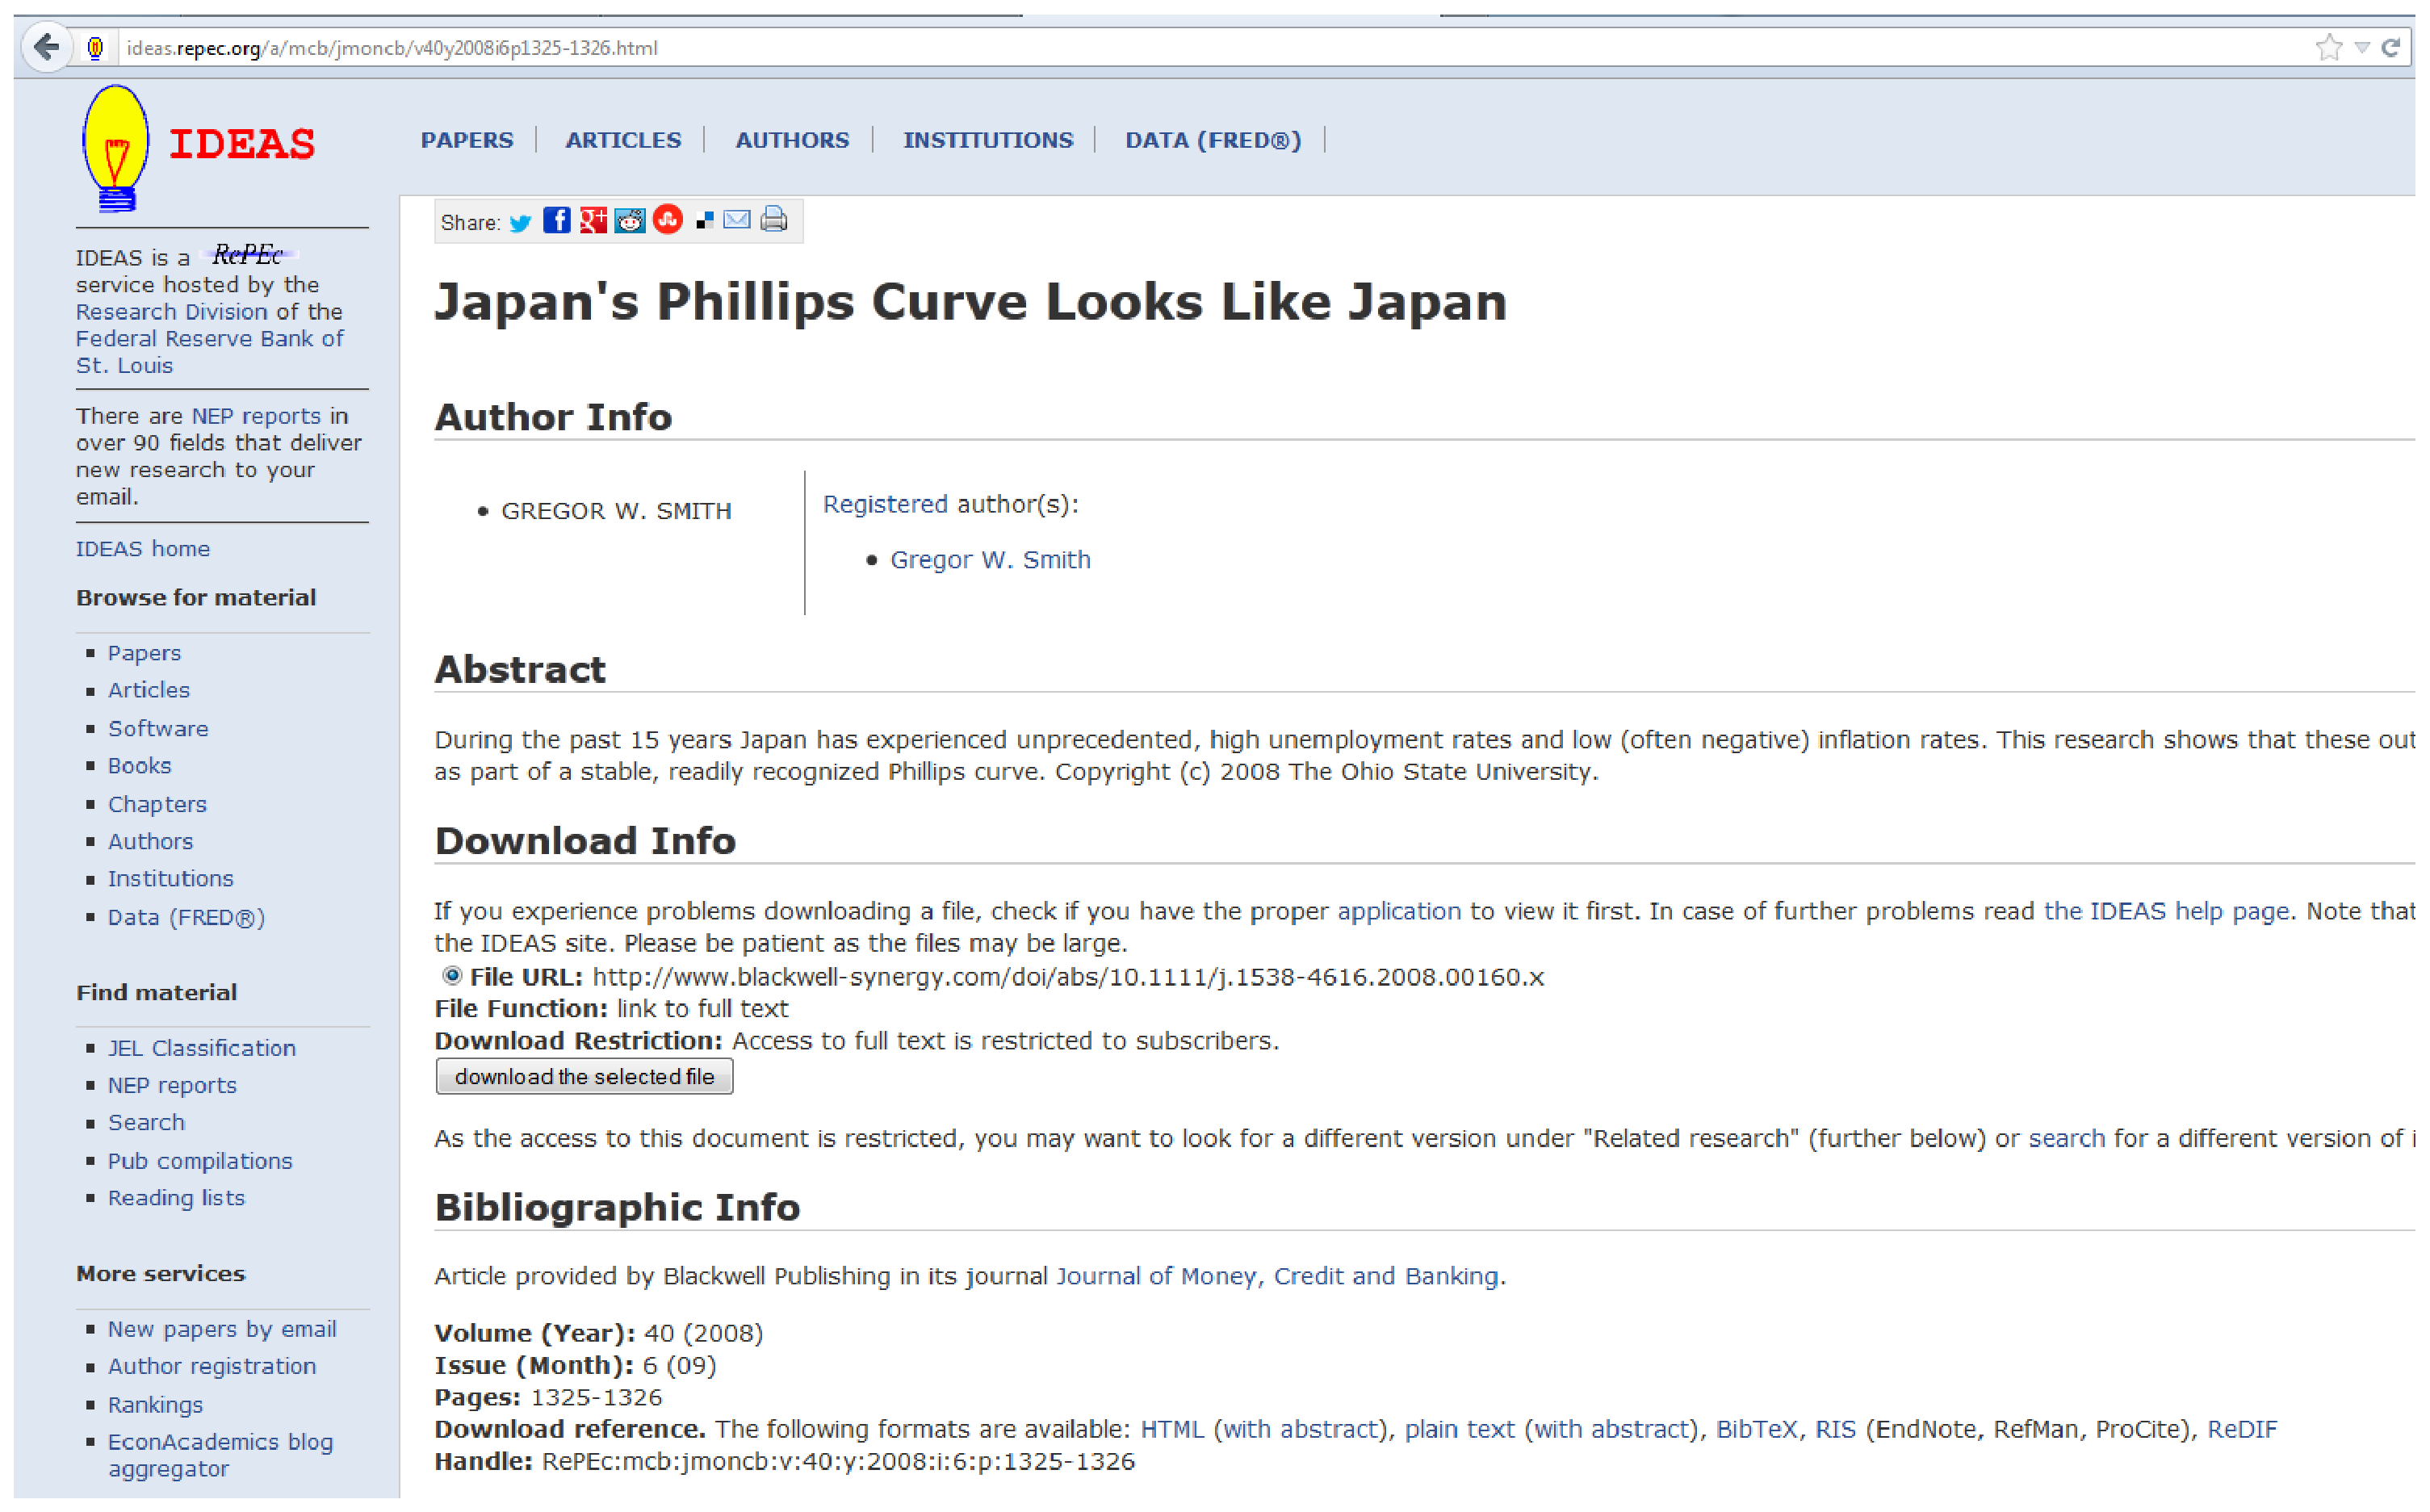
\includegraphics[width=1.0\linewidth]{Ideas} %um die Bilddatei Ideas einzubinden muss sie im gleichen Ordner wie dieses Dokument vorhanden sein
    \end{minipage}
    \begin{minipage}{0.3\linewidth}
        \begin{enumerate} %enumerate generiert eine nummerierte Aufzählung
            \item Dies ist ein bisschen Text...
            \item Dies ist noch mehr Text
        \end{enumerate}
    \end{minipage}
\end{figure}

\clearpage

\section{Referenzen und Zitationen mit \LaTeX}
Referenzen sollten mit Bib\LaTeX\ verwaltet werden. Die bibliographischen Informationen werden in einer \texttt{.bib}-Datei gespeichert, für dieses in der Datei \texttt{mybibfile.bib}. Es handelt sich um eine Text-Datei, die Sie auch manuell bearbeiten können. Es empfiehlt sich aber die Verwendung einer Literaturverwaltungssoftware. Ein gutes GUI-interface für Windows ist JabRef. Laden Sie es auf \url{http://jabref.sourceforge.net/} herunter. Wie in Abbildungen \ref{fig:Ideas1} und \ref{fig:Ideas2} gezeigt, können Sie die bibliographischen Informationen zu vielen Referenzen, die Bib\LaTeX\ benötigt, auf \url{https://ideas.repec.org} oder von Datenbanken wie JSTOR, ScienceDirect oder Google Scholar herunterladen. Kopieren Sie einfach den Bib\TeX-Quellcode und fügen ihn in Jabref wie in Abbildung \ref{fig:jabref} ein. Versuchen Sie, aussagekräftige und eindeutige Bib\TeX-keys zu verwenden, z.B.\ verwenden Sie \textit{Smith2006} anstelle von \textit{Reference1} (oder noch besser \textit{Smith2006Japan}).

\begin{figure}[h!] % h! platziert das float-Objekt an diese Stelle im Dokument, nutzen Sie t um das Objekt oben auf der Seite zu platzieren, b für unten, p um es auf einer gesonderten Seite zu platzieren. Diese Optionen können in Kombination verwendet werden, um eine Präferenzenfolge zu spezifizieren
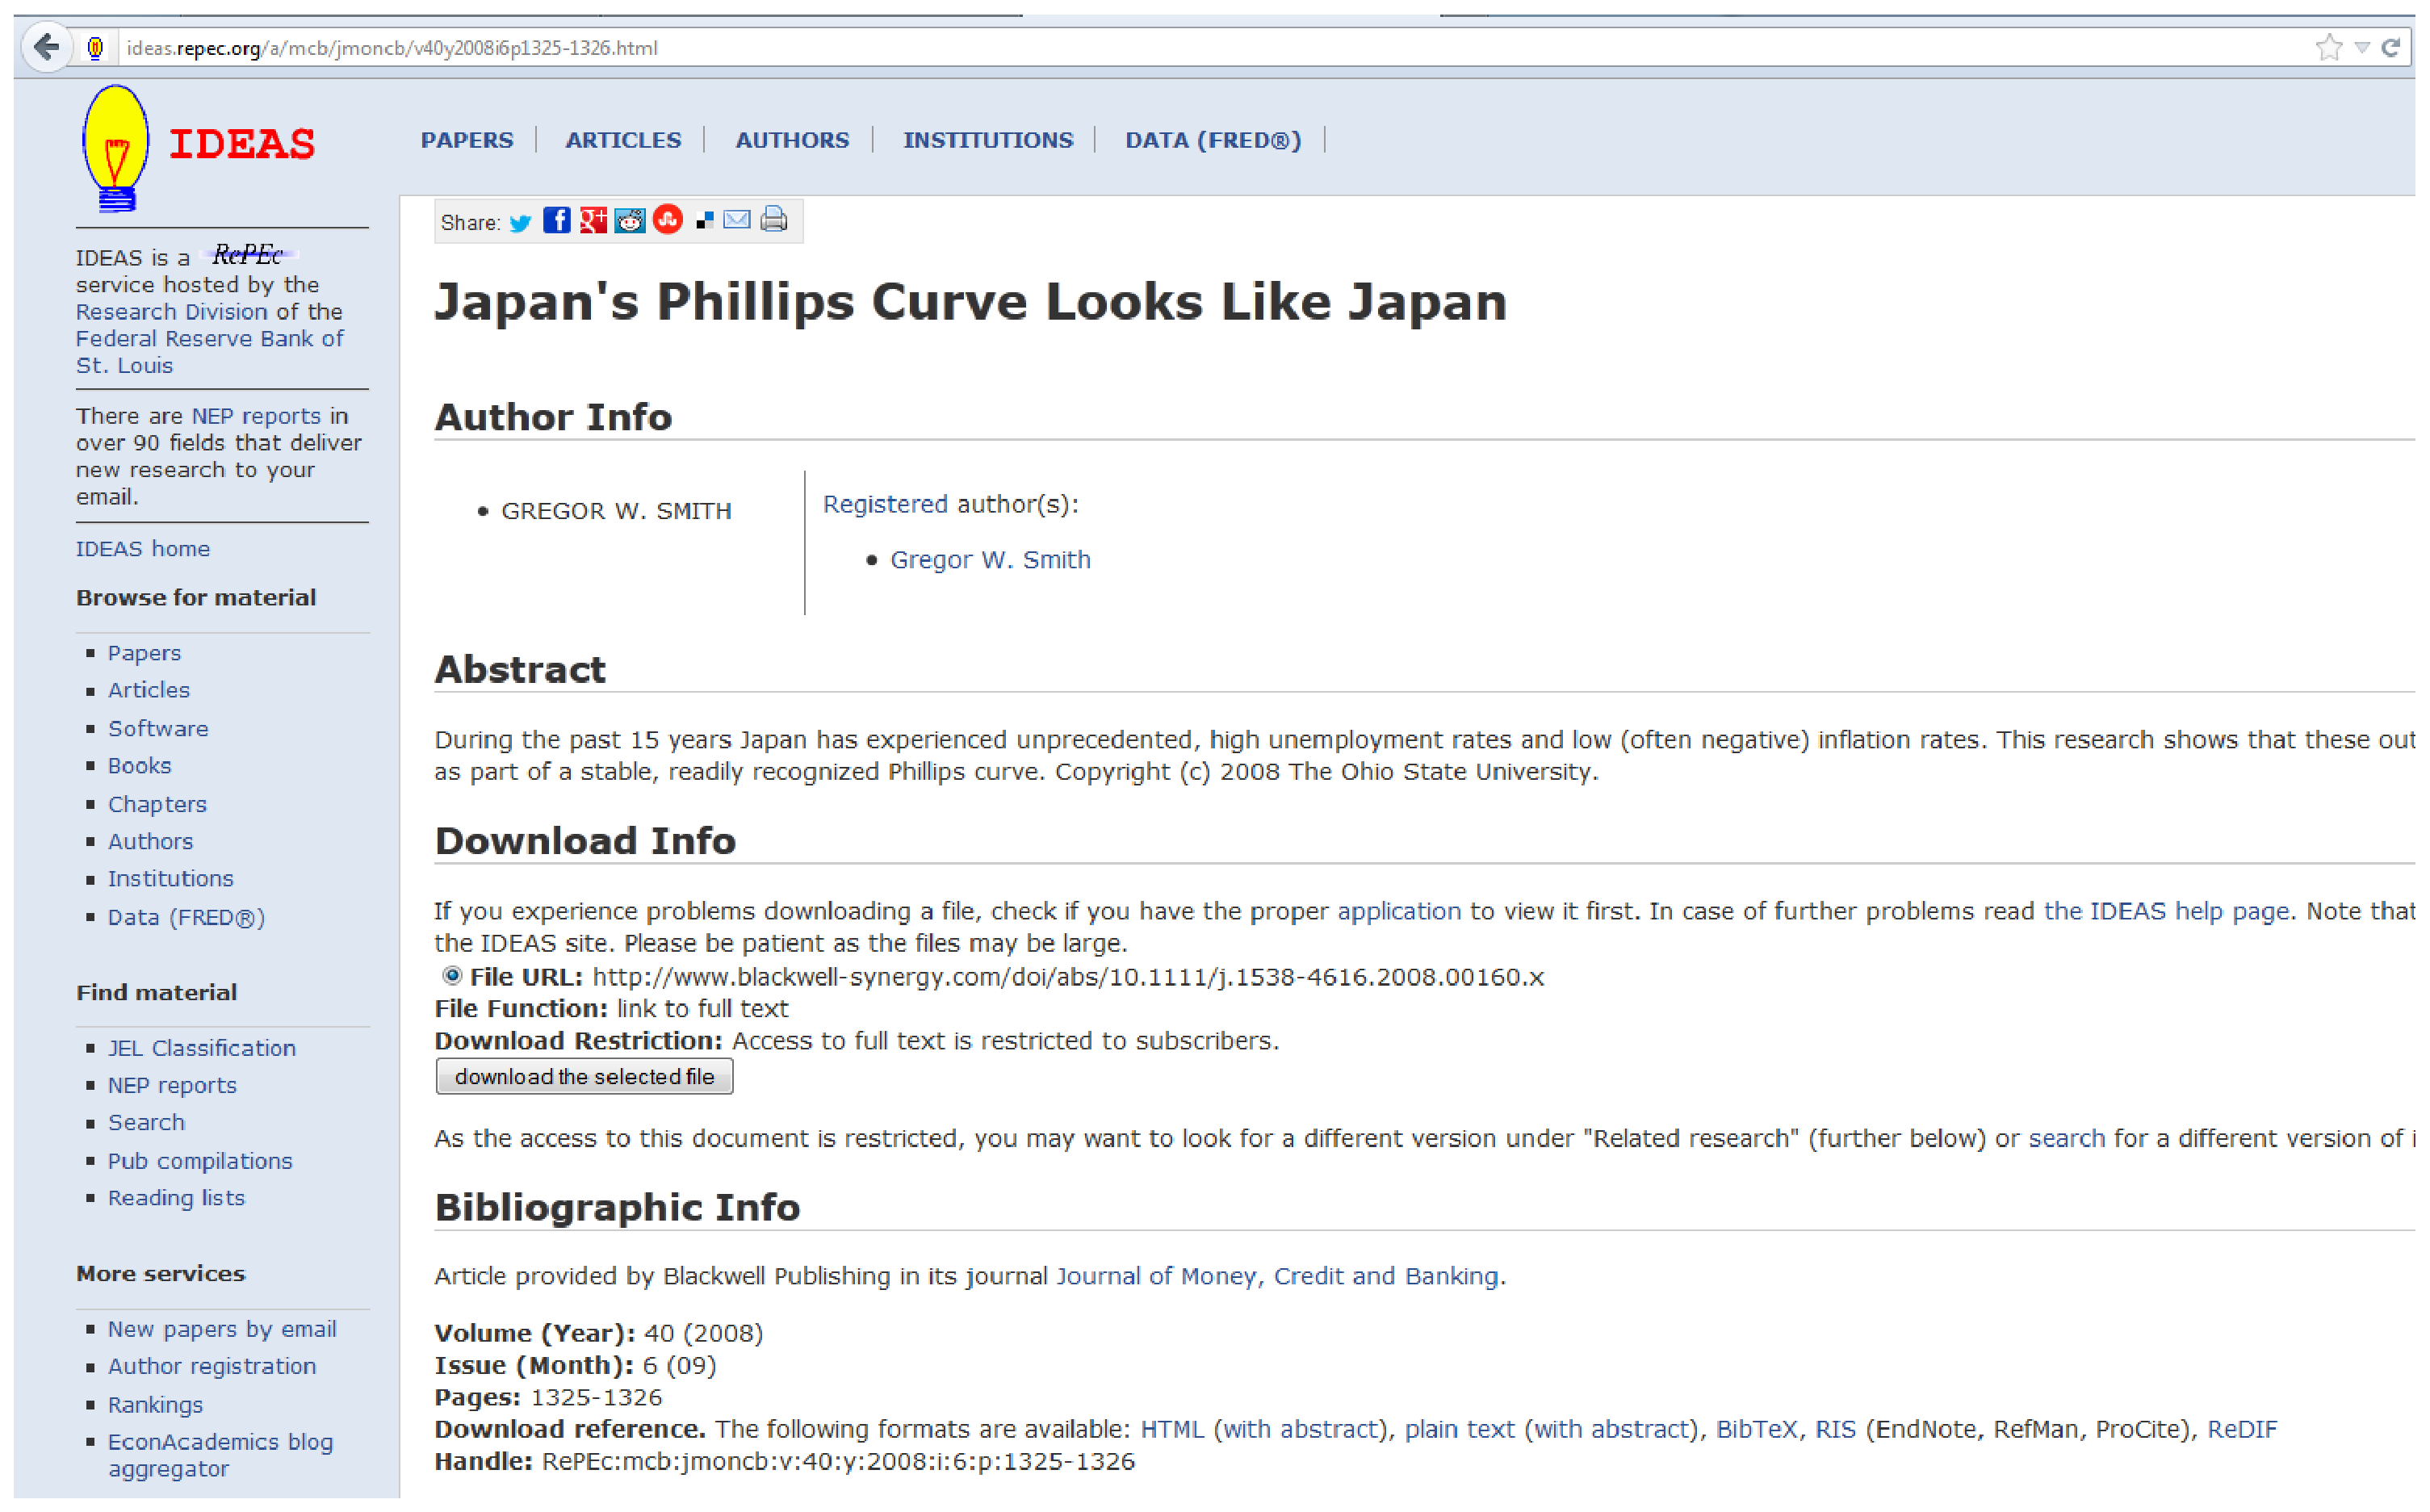
\includegraphics[scale=0.3]{Ideas}  % skaliert die Abbildung auf 35%
\caption[Titel für Abbildungsverzeichnis]{Um die bibliographischen Informationen von Repec herunterzuladen, klicken Sie auf \emph{Download reference: Bibtex}}\label{fig:Ideas1} %label, um später auf diese Abbildung zu verweisen
\end{figure}

\begin{figure}[t!]
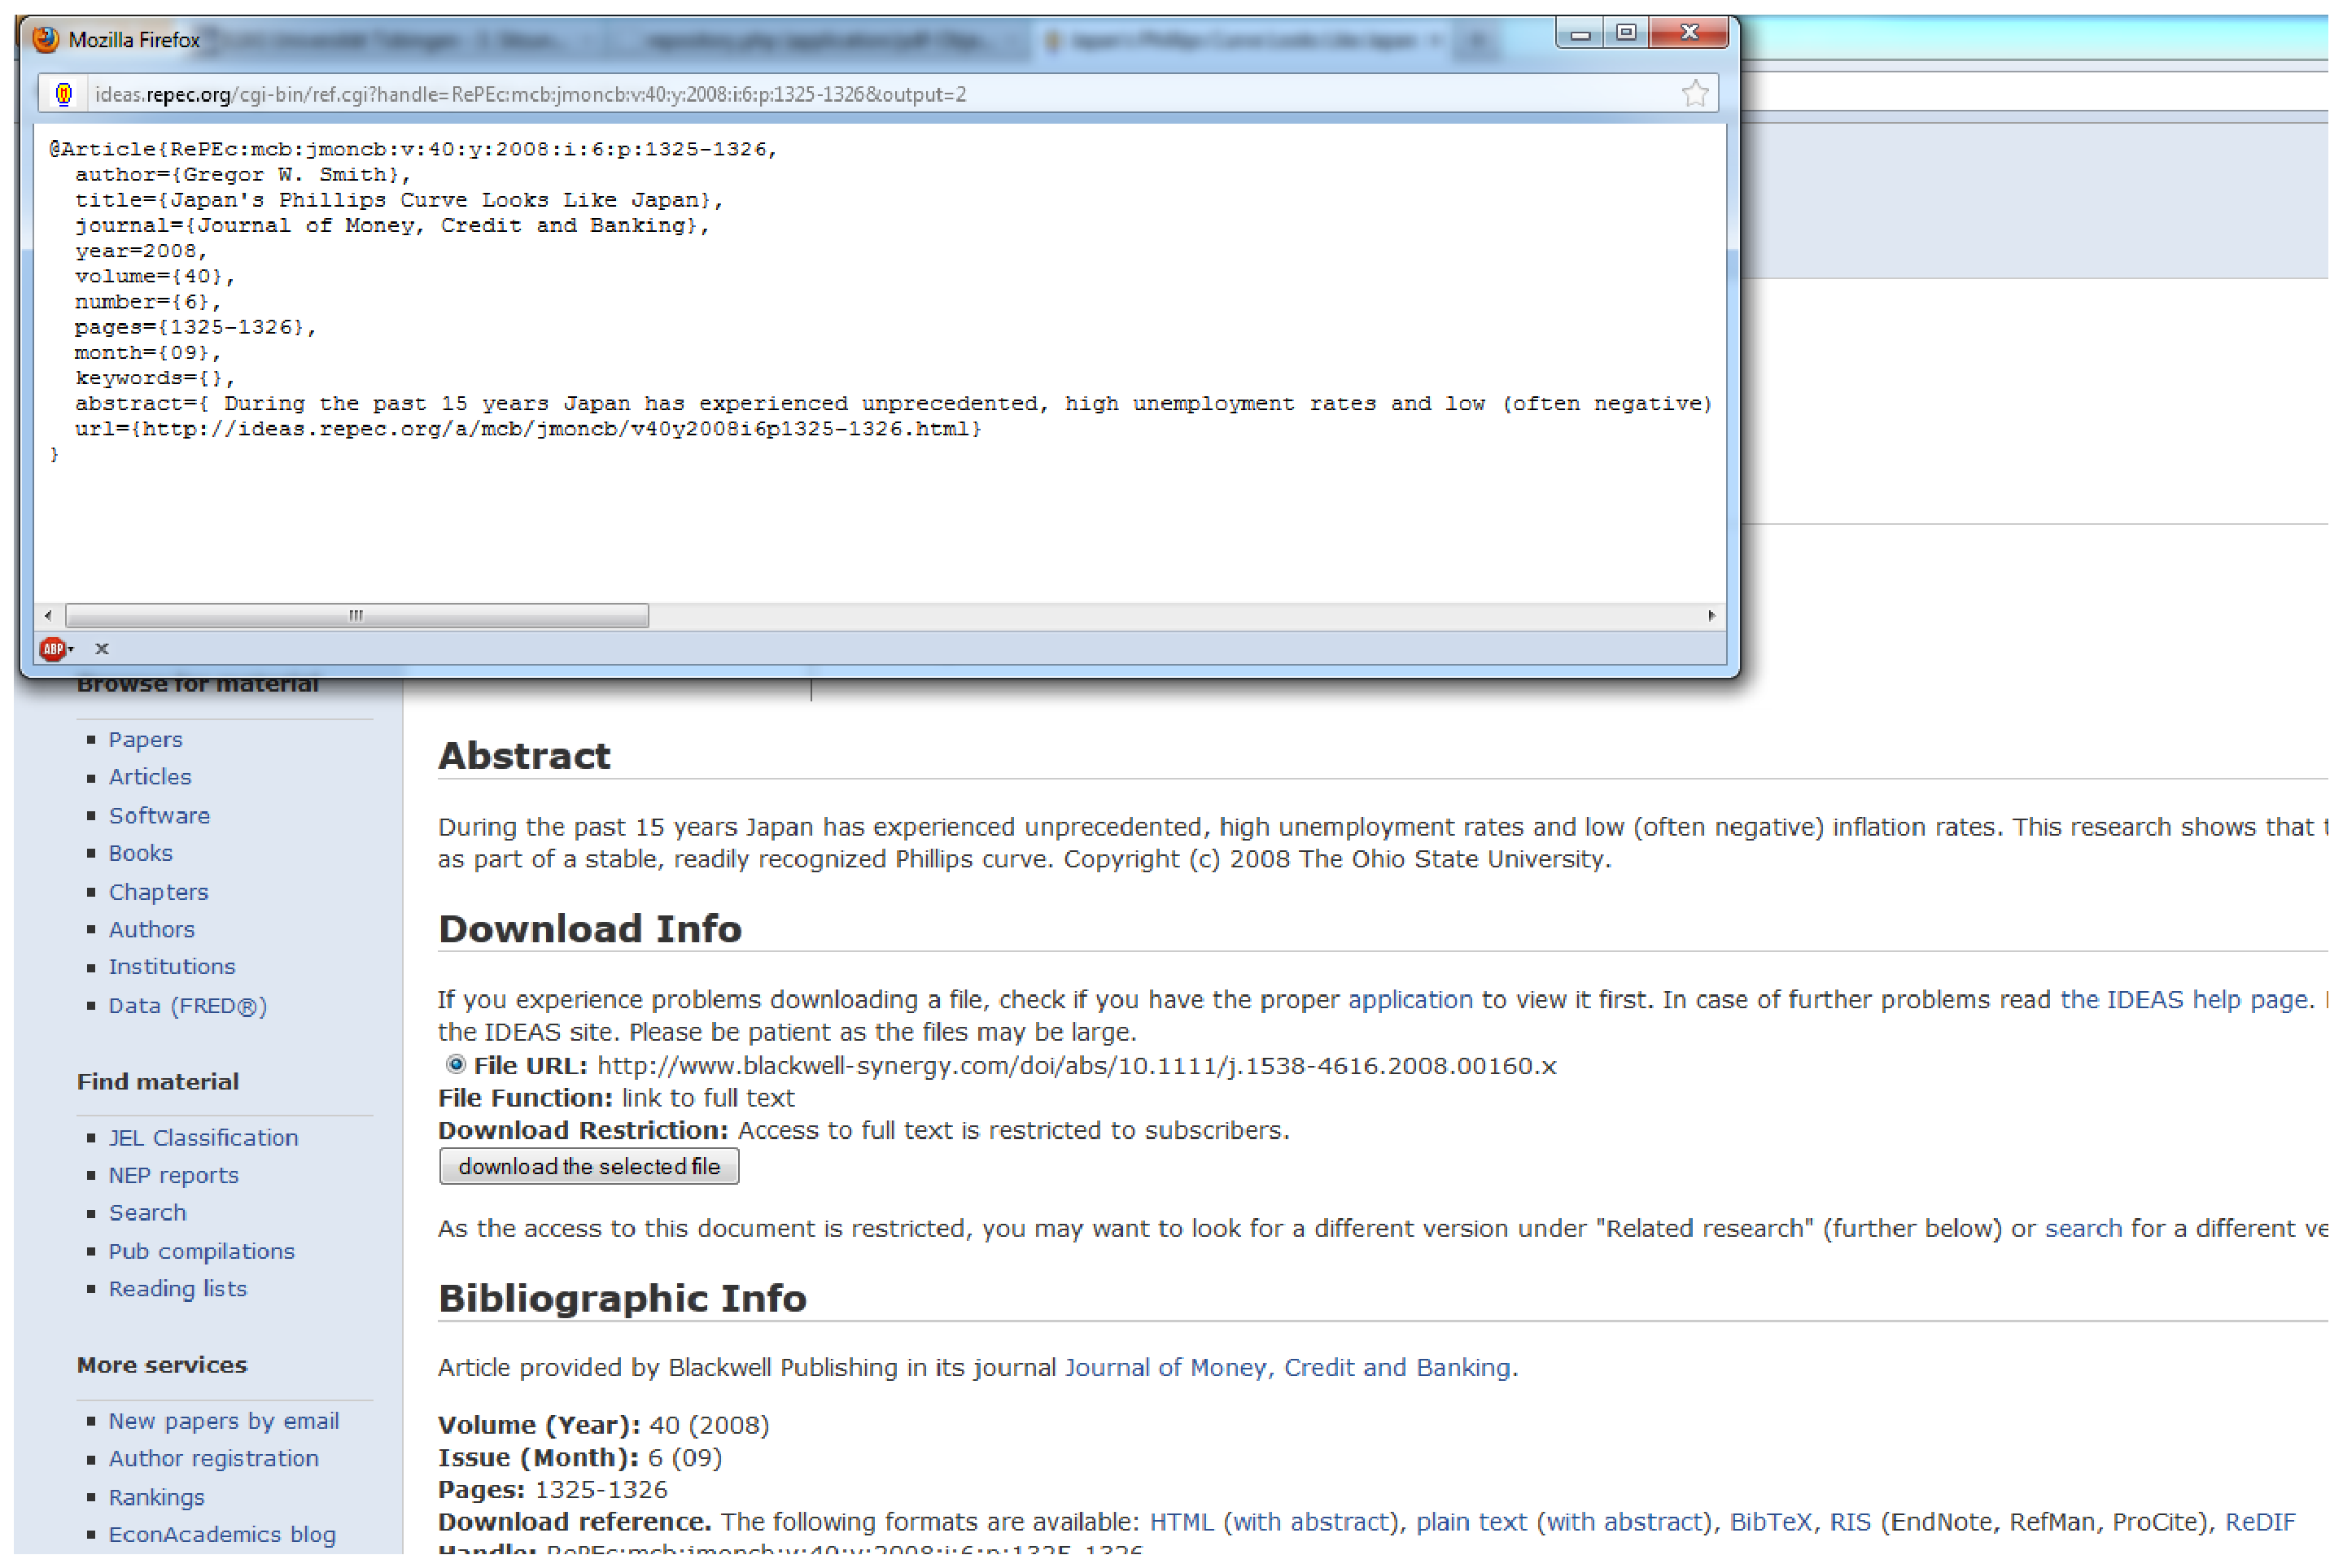
\includegraphics[width=\ScaleIfNeeded]{Ideasbibtex}
\caption[Referenz von Bibtex entnehmen]{Kopieren Sie den Text aus dem Fenster}\label{fig:Ideas2}
\end{figure}
%
\begin{figure}[t!]
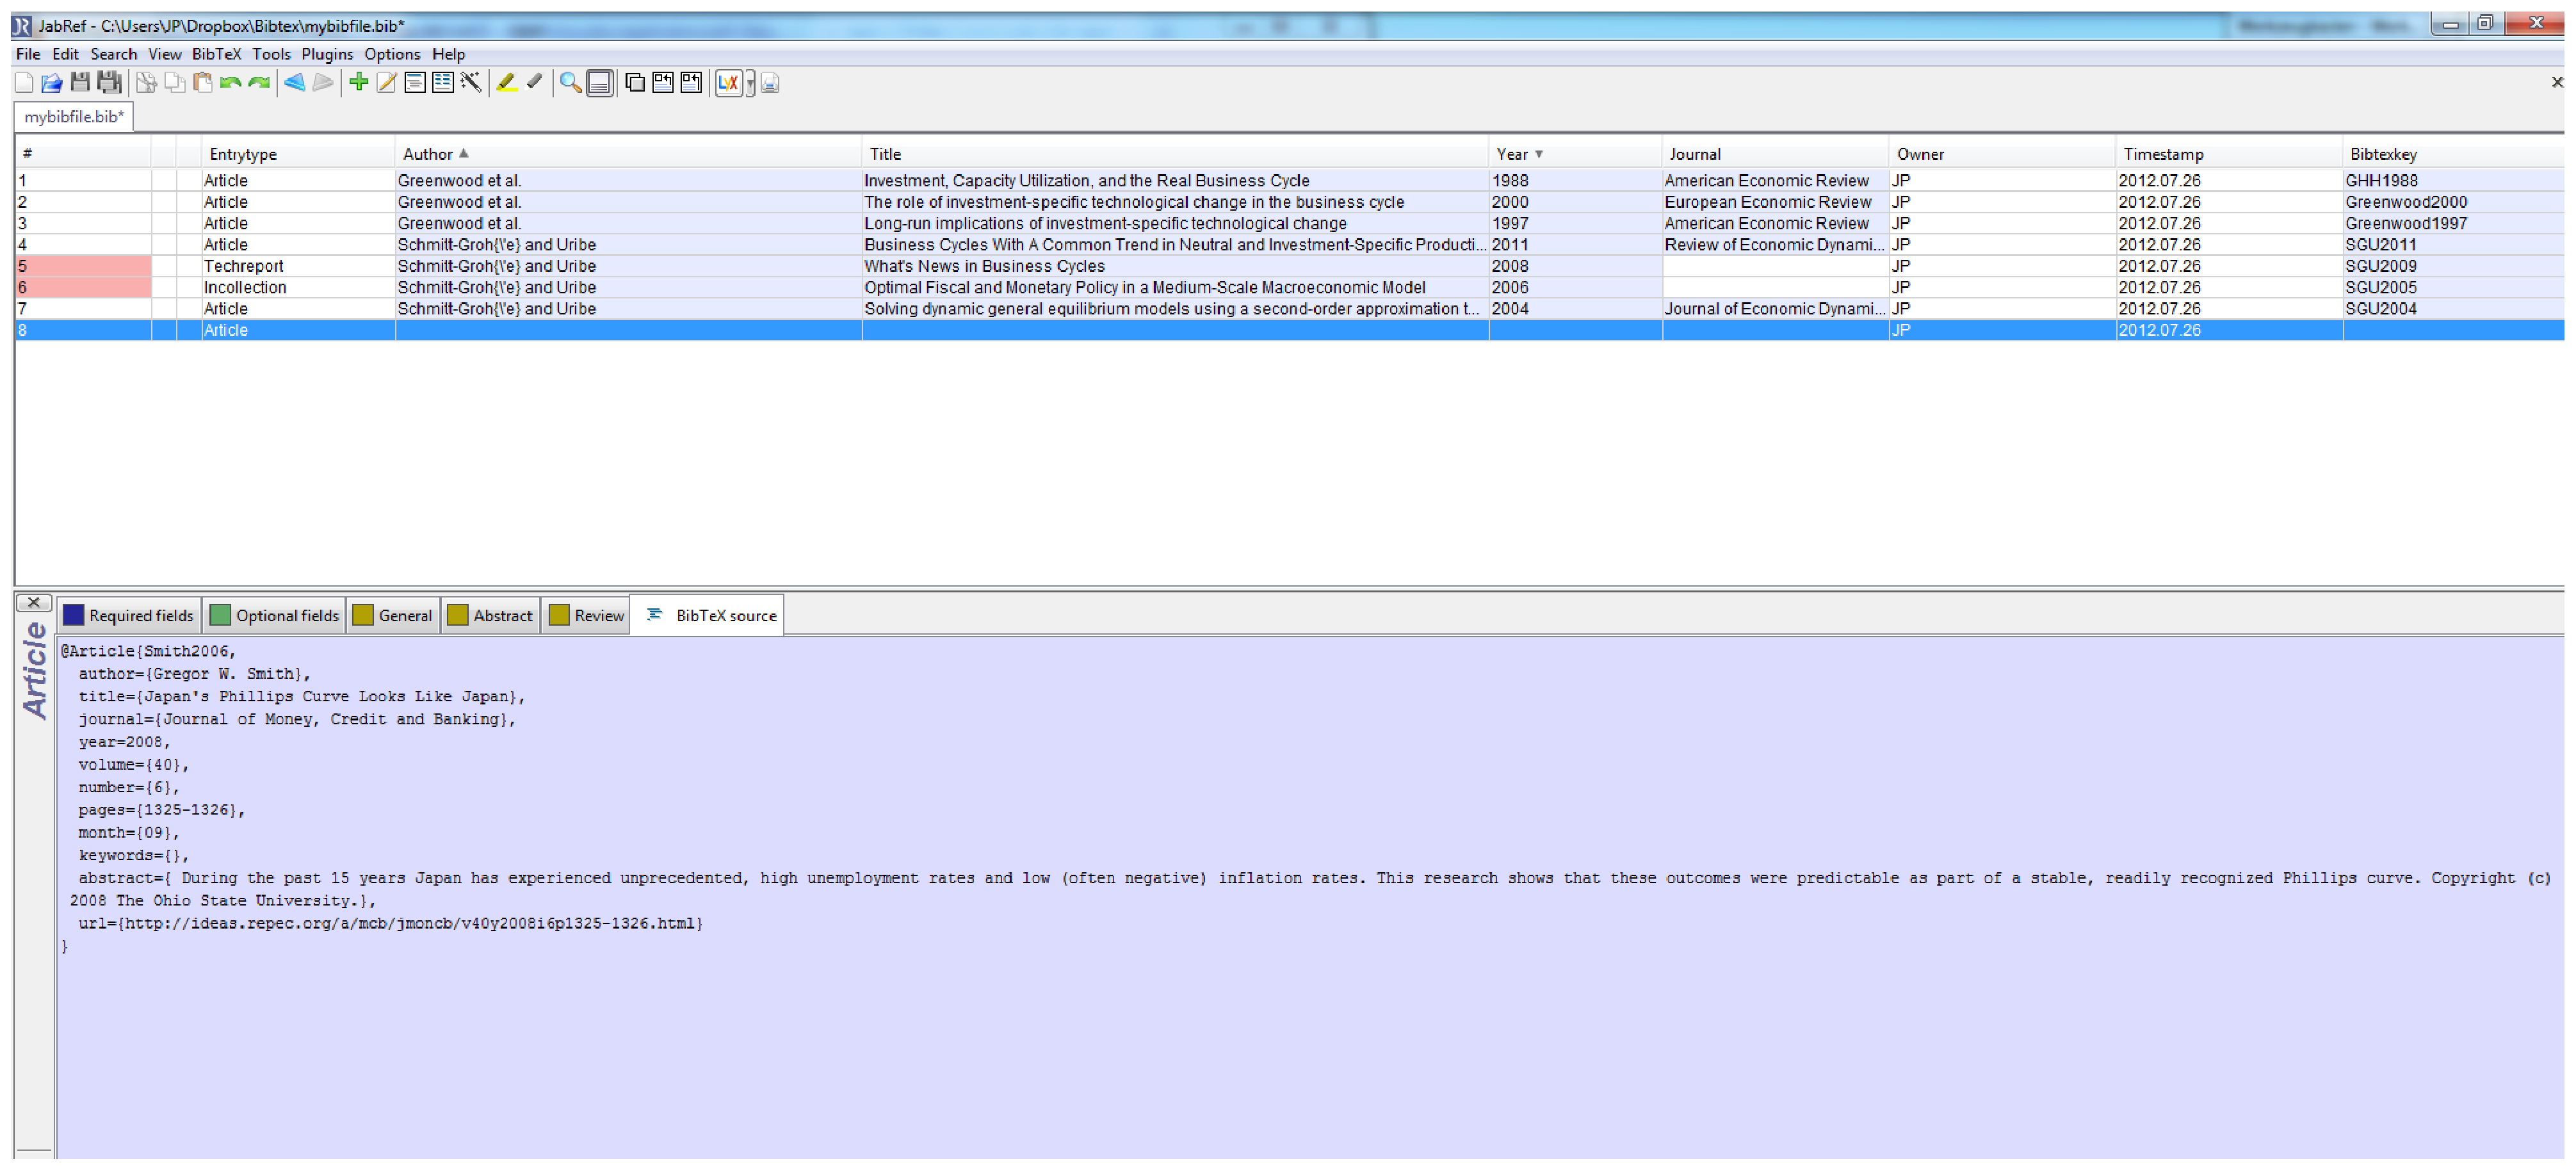
\includegraphics[width=\ScaleIfNeeded]{JabrefAdd}
\caption[Nutzung von JabRef]{Klicken Sie auf den Add-Button (grünes Plus) und fügen Sie den kopierten Text unter \emph{Bibtex Source} ein. Vergessen Sie nicht den Bibtex-key anzupassen. Hier habe ich den Key \texttt{Smith2006} gewählt}\label{fig:jabref}
\end{figure}


Bitte zitieren Sie im Text und nicht in Fußnoten.\interfootnotelinepenalty=5000\footnote{Wie Sie sehen, werden Fußnoten mit dem \texttt{\textbackslash footnote{}}-Befehl eingefügt. Manchmal können Fußnoten sehr lang werden. In diesem Fall teilt \LaTeX\ die Fußnote automatisch auf mehrere Seiten auf. Manchmal funktioniert diese automatische Einstellung nicht wie gewollt. Sie können sie durch \texttt{\textbackslash interfootnotelinepenalty=x} verändern, wobei $x$ eine ganze Zahl zwischen $0$ und $10{.}000$ ist, mit 100 als Standardwert. Wenn $10{.}000$ eingestellt ist, teilt \LaTeX\ die Fußnote nicht. Die Option \texttt{\textbackslash interfootnotelinepenalty=x} kann sowohl in der Präambel definiert werden, um sich auf alle Fußnoten zu beziehen oder im Text direkt für eine Fußnote. Nach dieser Fußnote muss der Wert wieder auf den Standardwert zurückgesetzt werden, wenn Sie dadurch nur diese eine Fußnote beeinflussen wollen.}\interfootnotelinepenalty=100\textsuperscript{,}\footnote{Für weitere Bib\LaTeX-Befehle besuchen Sie \url{http://mirror.ctan.org/macros/latex/contrib/biblatex/doc/biblatex.pdf}.} Der Befehl \texttt{\textbackslash textcite\{Smith2006\}}, wobei \textit{Smith2006} der in JabRef definierte Bibtex-Key ist, zitiert die Referenz mit Namen: \textcite{Smith2006}. Der Befehl \texttt{\textbackslash parencite\{Smith2006\}} zitiert die Referenz in Klammern: \parencite{Smith2006}. Der Befehl \verb|\parencite[Prefix][Suffix]{Smith2006}| fügt Präfixe und Suffixe in der Klammer ein: \parencite[see e.g.][pp. 1-4]{Smith2006}.\\

\begin{figure}[t]
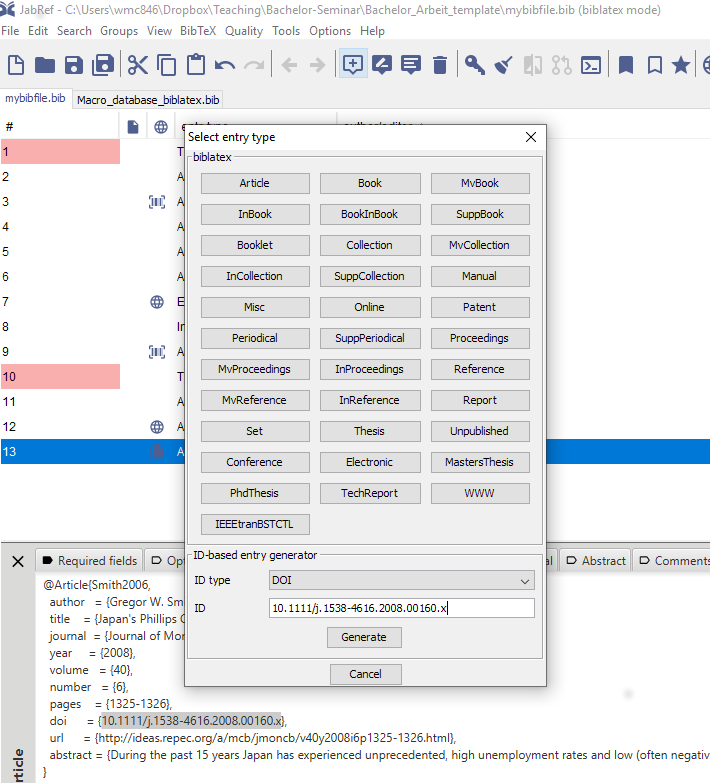
\includegraphics[width=\ScaleIfNeeded]{JabrefDOI}
\caption[Nutzung von DOIs in JabRef]{Klicken Sie auf den Add-Button (grünes Plus) und tragen Sie den Digital Object Identifier (DOI) eines Artikeln ein, um einen entsprechenden Eintrag hinzuzufügen.}\label{fig:jabref_doi}
\end{figure}
Bib\LaTeX verkürzt automatisch wiederholte Zitationen des gleichen Autors, z.B.\ \parencite{SGU2004JET,SGU2004,SGU2009,SGU2011} und liefert korrekte Referenzen mit a,b, etc. Außerdem erfüllt es verschiedene bibliographische Anforderungen von Zeitschriftenartikeln wie \textcite{SGU2004} und Büchern wie z.B.\ \textcite{SGU2005}.\\
Seitenbereiche wie \textcite[][99\psq]{Gali2015book} und \textcite[][99\psqq]{Gali2015book} werden mit den Befehlen \texttt{\textbackslash psq} und \texttt{\textbackslash psqq} eingefügt, z.B.\ \texttt{\textbackslash textcite[][99\textbackslash psqq]\{Gali2015book\}} erzeugt \textcite[][99\psqq]{Gali2015book}. Beachten Sie, dass Sie nur die Seitenzahl 99 angeben und nicht auch ``S.''. Dies stellt sicher, dass Bib\LaTeX\ automatisch ``p.'' verwendet, wenn Sie die Sprache des Dokumentes über \texttt{babel} auf Englisch ändern.
Es gibt auch multicite-Befehle wie \verb|\parencites|, die es erlauben für jede Zitation ein Präfix und Suffix zu definieren. So erzeugt \verb|\parencites[vgl.][99\psq]{Gali2015book}[][122\psqq]{SGU2011}| den Eintrag \parencites[vgl.][99\psq]{Gali2015book}[][122\psqq]{SGU2011}.


Der Stil des Literaturverzeichnisses wird mittels der \verb|bibstyle|-Option festgelegt. Diese Vorlage nutzt die JME-Stil-Vorlage aus der Datei \texttt{JME.bbx}. Daher benötigen Sie diese Datei, um das Dokument zu kompilieren.

Wie in Abbildung \ref{fig:jabref_doi} gezeigt, können Sie Einträge für veröffentlichte Artikel auch sehr leicht auf Basis der Digital Object Identifier (DOI) erstellen.

Sie können Bib\TeX-Einträge auch aus Google Scholar exportieren. Jedoch ist diese Funktion standardmäßig deaktiviert und muss erst in den Einstellungen aktiviert werden (siehe Abbildung \ref{fig:scholar}). Zudem sind die Einträge in Google Scholar oft weniger zuverlässig und müssen streng kontrolliert und überarbeitet werden. Achten Sie zudem darauf, dass Sie die richtige Version exportieren, d.h.\ z.B.\ die veröffentlichte Fassung eines Artikels und nicht die Arbeitspapierversion.

\begin{figure}[th!]
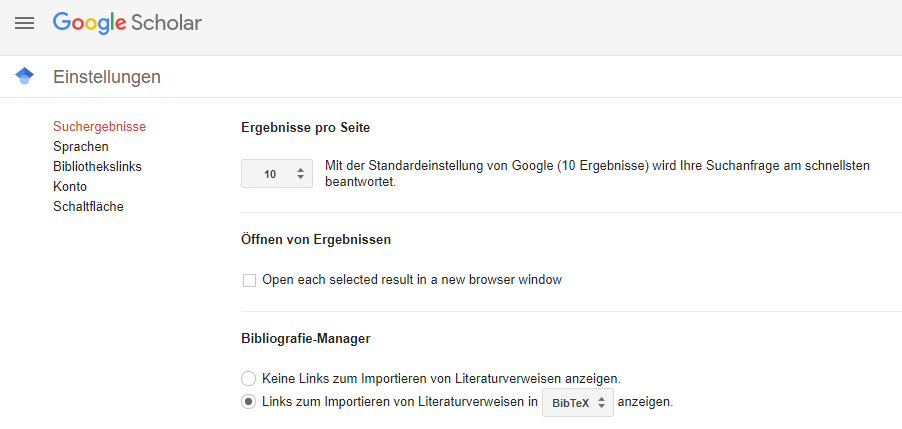
\includegraphics[width=16cm]{Scholar}
\caption[Google Scholar]{Um Bib\TeX-Einträge aus Google Scholar zu exportieren, müssen Sie dieses Feature in den Einstellungen aktivieren.}\label{fig:scholar}
\end{figure}

Für elektronische Quellen wie Blog-Einträge \parencite[e.g.\ ][]{Krugman2012} sollten Sie den Typ \texttt{electronic} in JabRef verwenden. Leider müssen Sie manuell das \texttt{urldate}-Feld der Bib\TeX-source hinzufügen um das Besuchsdatum anzuzeigen, wie in Abbildung \ref{fig:jabref_urldate} gezeigt. Das Datenformat ist JJJJ-MM-TT.

\begin{figure}[t!]
\includegraphics[width=\ScaleIfNeeded]{Urldate}
\caption[Einfügen von elektronischen Quellen]{Bei elektronischen Quellen, müssen Sie manuell das \texttt{urldate}-Feld der Bib\TeX-source hinzufügen.}\label{fig:jabref_urldate}
\end{figure}

Viele Bibliographie-Stilformate stellen besondere Anforderungen an die Kapitalisierung von Artikel-Titeln. Daher ist es sinnvoll, die Titel nicht manuell zu kapitalisieren. In diesem Fall ist es notwendig, Bib\LaTeX\ zu instruieren, welche Teile eines Titels immer kapitalisiert werden. Denn die Eingabe von\\
\texttt{title     = \{ABCs (and Ds) of understanding VARs}\}\\
würde bei einem nicht kapitaliserten Format in ``abcs (and ds) of understanding vars'' resultieren. Mithilfe von geschweiften Klammern lässt sich definieren, welche Teile verbatim übernommen werden sollen. So resultiert\\
\texttt{title     = \{\{ABC\}s (and \{D\}s) of understanding \{VAR\}s\}}\\
im gewünschten ``ABCs (and Ds) of understanding VARs''. Dieser Trick lässt sich auch bei Autorennamen verwenden, z.B.\ sorgt
\texttt{author     = \{Wouter \{Den Haan\}\}}\\
dafür, dass Bib\LaTeX\ nicht denkt, der Nachname wäre nur Haan. Allerdings ist generell das Format Nachname, Vorname zu bevorzugen:
\texttt{author     = \{Den Haan, Wouter\}}\\


\clearpage


\section{Symbol- und Abkürzungsverzeichnis}
Ein Verzeichnis für Symbole und eines für Abkürzungen wie am Anfang dieses Dokuments kann mithilfe des \texttt{glossaries} Pakets erstellt werden.\footnote{Weitere Informationen finden Sie auf \url{http://mirror.ctan.org/macros/latex/contrib/glossaries/glossariesbegin.pdf} (Beginner's guide) und auf \url{http://mirror.ctan.org/macros/latex/contrib/glossaries/glossaries.pdf}.} Wenn Sie TeXnicCenter nutzen, müssen Sie manuell makeindex einfügen.\footnote{Siehe \url{http://brianhoffmann.de/journal/thesis/2011-08-01/latex-glossaries-with-texniccenter/} oder \url{https://tex.stackexchange.com/questions/153323/acronyms-glossaries-not-being-output-in-the-pdf/}.}

\subsection{Das \texttt{glossaries} Paket in der Präamble}
Das \texttt{glossaries} Paket ist eines der wenigen Pakete, die nach dem \texttt{hyperref}-Paket geladen werden müssen. In dieser Vorlage habe ich das Standardglossar für Abkürzungen verwendet. Zusätzlich habe ich ein zweites Glossar für das Symbolverzeichnis definiert und mit dem Label \texttt{symbolslist} versehen. Dies erreicht der folgende Befehl\\
\verb|\newglossary[slg]{symbolslist}{syi}{syg}{List of Symbols}|.\\

Nach Definition der Glossare muss \verb|\makeglossaries| folgen, damit die Glossareinträge sortiert werden können.\\

Der folgende Befehl gibt das Abkürzungsverzeichnis aus\\
\verb|\printglossary[type=\acronymtype,style=long]|.\footnote{Natürlich kann der Stil verändert werden.}\\
Der folgende Befehl gibt das Symbolverzeichnis aus\\
\verb|\printglossary[type=symbolslist,style=long,title=List of Symbols]|.

\subsection{Definieren und nutzen von Verzeichniseinträgen}
Die Einträge der Glossare können entweder in der Präamble oder im Haupttext definiert werden. Zum Beispiel definiert der Befehl\\
\verb|newglossaryentry{symb:pi}{name={\ensuremath{\pi}}...|\\
in der Präambel dieses Dokuments einen Eintrag für das Glossar \texttt{symbolslist}. Allerdings erscheint das Symbol \gls{symb:pi} nicht im Symbolverzeichnis, wenn es im Text nicht genutzt wird. Normalerweise geschieht dies durch einen Verweis mithilfe des \verb|\gls{}|-Befehls. Zum Beispiel gibt \verb|\gls{symb:pi}| \gls{symb:pi} aus. Dieser Befehl kann auch folgendermaßen in Gleichungen genutzt werden

\begin{equation}
	\gls{symb:e}^{\gls{symb:i}\gls{symb:pi}}-1=0 \;.
\end{equation}


\newacronym{acro:DSGE}{DSGE}{Dynamic Stochastic General Equilibrium} %Definiert eine Abkürzung im Haupttext

Sie können Symbole und Abkürzungen auch im Haupttext definieren, z.B.\ indem Sie\\
\verb|\newacronym{acro:DSGE}{DSGE}{Dynamic Stochastic General Equilibrium}|\\
an den Anfang oder das Ende eines Abschnittes stellen, in welchem Sie die Abkürzung zum ersten mal benutzten. Anschließend können Sie die Abkürzung mit \verb|\gls{}| nutzen, z.B.\ \verb|\gls{acro:DSGE}|. Beim ersten Aufrufen einer Abkürzung gibt \LaTeX\ automatisch die lange Version gefolgt von der Abkürzung aus. Ab dem zweiten mal wird nurnoch die Abkürzung ausgegeben. Zum Beispiel wird \gls{acro:DSGE} von nun an mit \gls{acro:DSGE} abgekürzt. Außerdem werden alle Symbole und Abkürzungen, die mit \verb|\gls{}| aufgerufen werden, dem entsprechenden Verzeichnis hinzugefügt.\\
\textbf{Um Glossare korrekt zu aktualisieren müssen Sie \LaTeX\ normalerweise mindestens zwei mal ausführen.}\\

Wenn Sie nicht alle Möglichkeiten von glossaries ausschöpfen möchten, können Sie das Symbol oder die Abkürzung, die Sie benötigen, auch einfach in der Präambel definieren und sie dem entsprechenden Verzeichnis mithilfe von \verb|\glsadd{}| nach der Definition zuordnen (wie hier geschehen mit \verb|\glsadd{OLS}|). Der große Nachteil hierbei ist, dass manuell dafür gesorgt werden muss, dass nur Abkürzungen und Symbole in den Verzeichnissen auftauchen, die auch im Text vorkommen.



\clearpage

\section{Weitere Informationen zu \LaTeX}

\begin{itemize}
	\item Fast jede erdenkliche \LaTeX-Frage wurde schonmal gefragt. Nutzen Sie Google oder durchsuchen Sie die FAQ auf \url{https://texfaq.org/}
	\item Es gibt fatale \LaTeX\ Fehler, die Sie niemals machen sollten, Siehe \url{https://ctan.org/tex-archive/info/l2tabu/german?lang=de}.
	\item Viel hilfreiches finden Sie auf \url{http://en.wikibooks.org/wiki/LaTeX/}.
	\item Für Präsentationen können Sie \LaTeX\ Beamer nutzen, Siehe \url{ftp://ftp.fu-berlin.de/tex/CTAN/macros/latex/contrib/beamer/doc/beameruserguide.pdf}.
\end{itemize}

%_________________ Ende des Haupttexts_________________%

\clearpage

%_________________ Literaturverzeichnis _______________%

\phantomsection  \label{sec:literatur}                                 % stellt eine korrekte Verbindung zum Inhaltsverzeichnis sicher
\addcontentsline{toc}{section}{Literaturverzeichnis}        % fügt die Zeile Literaturverzeichnis dem Inhaltsverzeichnis hinzu
\onehalfspacing


\printbibliography % Ausgabe des Literaturverzeichnisses mithilfe von BibLaTeX



\clearpage
%_________________ Zusätzliches Material _______________%
\appendix
\numberwithin{equation}{section} % startet Seitennummerierung wieder bei 1
\numberwithin{table}{section}
\numberwithin{figure}{section}

\section{Appendix 1}

Informationen präsentiert im Appendix.
\begin{equation}
    MV=PQ
\end{equation}

\clearpage

\section{Ergänzende Tabellen}


\begin{table}[h!] % h! platziert das float Objekt an diese Stelle, nutze t für oben auf der Seite, b für unten
\caption{Titel der Tabelle}
\label{tab:SuppTable1}
\centering
 \begin{tabular}{lcr}
   Noch & eine & Tabelle\\
\toprule
   left aligned & centered & right aligned \\
   \multicolumn{2}{c}{Text über zwei Spalten} & Dritte Spalte \\
\bottomrule
\end{tabular}
\caption*{\footnotesize{\emph{Notes:} Fügen Sie hier eine Beschreibung hinzu}}
\end{table}

\clearpage

\section{Eidesstattliche Versicherung/Affidavit}

Hiermit versichere ich, dass ich die vorliegende Arbeit selbständig und ohne fremde Hilfe verfasst, die Zitate ordnungsgemäß gekennzeichnet habe und keine anderen, als die im Literatur/Schriftenverzeichnis angegebenen Quellen und Hilfsmittel benutzt wurden.

Ferner habe ich vom Merkblatt über die Verwendung von Bachelor- und Abschlussarbeiten Kenntnis genommen und räume das einfache Nutzungsrecht an meiner Bachelorarbeit der Universität der Bundeswehr München ein / nicht ein.

\vspace{3cm}
\makebox[\textwidth]{\hrulefill \hspace{3cm} \hrulefill}

Ort, Datum/Place, Date \hfill Unterschrift/Signature


\end{document}




